\documentclass[12pt]{beamer}

\usetheme{Air}
\usepackage{graphics}
\usepackage{graphicx}
%\usepackage{amsthm}
\usepackage{thumbpdf}
\usepackage{wasysym}
\usepackage{ucs}
\usepackage[utf8]{inputenc}
\usepackage{pgf,pgfarrows,pgfnodes,pgfautomata,pgfheaps,pgfshade}
\usepackage{verbatim}
\usepackage{tikz}
\usepackage{pgfmath}
\usetikzlibrary{calc}
\usetikzlibrary{backgrounds}
\usetikzlibrary{arrows}
\usetikzlibrary{shapes.arrows}
\usetikzlibrary{shapes.geometric}
\usetikzlibrary{decorations.markings}
\usetikzlibrary{positioning}
\usetikzlibrary{fit,chains}

%\usepackage{pstricks}
%\newpsobject{psid}{psline}{linestyle=dotted,dotsep=1pt}
%\newpsobject{pspsi}{psline}{doubleline=true}
%\newpsobject{pssigma}{psline}{linewidth=1.5pt}

%\usepackage{pgfpages}
%\setbeamertemplate{note page}[plain]
%\setbeameroption{show notes on second screen=right}
%http://tex.stackexchange.com/questions/21777/is-there-a-nice-solution-to-get-a-presenter-mode-for-latex-presentations

\newcommand{\beq}{\begin{equation}}
\newcommand{\eeq}{\end{equation}}
\newcommand{\beqa}{\begin{eqnarray}}
\newcommand{\eeqa}{\end{eqnarray}}
\newcommand{\bi}{\begin{itemize}}
\newcommand{\ei}{\end{itemize}}
\newcommand{\ket} [1] {\vert #1 \rangle}
\newcommand{\bra} [1] {\langle #1 \vert}
\newcommand{\braket}[2]{\langle #1 | #2 \rangle}
\newcommand{\ev}[1]{\langle #1 \rangle}
\newcommand{\vbra}[1]{\left ( #1 \right |}
\newcommand{\vket}[1]{\left |#1 \right )}
\newcommand{\vbraket}[2]{\left ( #1 \middle |#2 \right )} 
\newcommand{\braopket}[3]{\left \langle #1 \middle |#2 \middle | #3 \right \rangle} 
\newcommand{\vbraopket}[3]{\left ( #1 \middle |#2 \middle | #3 \right )} 

%\newcommand<>{\highlighton}[1]{%
%  \alt#2{\structure{#1}}{{#1}}
%}

\newcommand{\icon}[1]{\pgfimage[height=1em]{#1}}

\usepackage{empheq}

\newlength\mytemplen
\newsavebox\mytempbox

\makeatletter
\newcommand\mybluebox{%
    \@ifnextchar[%]
       {\@mybluebox}%
       {\@mybluebox[0pt]}}

\def\@mybluebox[#1]{%
    \@ifnextchar[%]
       {\@@mybluebox[#1]}%
       {\@@mybluebox[#1][0pt]}}

\def\@@mybluebox[#1][#2]#3{
    \sbox\mytempbox{#3}%
    \mytemplen\ht\mytempbox
    \advance\mytemplen #1\relax
    \ht\mytempbox\mytemplen
    \mytemplen\dp\mytempbox
    \advance\mytemplen #2\relax
    \dp\mytempbox\mytemplen
    \fcolorbox{airlightblue}{white}{\hspace{1em}\usebox{\mytempbox}\hspace{1em}}}

\makeatother

\tikzset{peps/.style={circle=2pt,draw=black!100,fill=green!50,inner sep=3pt}}
\tikzset{bpeps/.style={circle=2pt,draw=black!100,thick,fill=green!50,inner sep=3pt}}
\tikzset{gamma/.style={circle=2pt,draw=black!100,fill=blue!20,inner sep=3pt}}
\tikzset{lambda/.style={rectangle,rotate=45,draw=black!100,fill=orange!50,inner sep=4pt}}
\tikzset{operator/.style={circle=2pt,draw=black!100,fill=orange!80,inner sep=3pt}}
\tikzset{cdot/.style={circle=2pt,draw=black!100,fill=white,inner sep=1pt}}
\tikzset{bg/.style={rounded corners,thin,fill=blue!10}}
\tikzset{inv/.style={opacity=0}}
\tikzset{spin/.style={circle=2pt,draw=black!100,fill=orange!80,inner sep=3pt}}
\tikzset{unitbox/.style={fill=black!3,rounded corners}}
\tikzset{corner/.style={rectangle=10pt,fill=blue!50,draw=black}}
\tikzset{side/.style={rectangle=6pt,fill=blue!20,draw=black}}
\tikzset{cside/.style={circle=6pt,fill=blue!20,draw=black}}
\tikzset{swapg/.style={circle=1pt,draw=black,fill=black!80,inner sep=1pt}}

\tikzset{base/.style={circle=2pt,fill=orange!80,draw=black}}
\tikzset{det/.style={circle=2pt,fill=blue!20,draw=black,inner sep=4pt}}
\tikzset{iso/.style={circle=2pt,fill=red!20,draw=black,inner sep=4pt}}
\tikzset{top/.style={circle=2pt,fill=black!20,draw=black,inner sep=4pt}}
\tikzset{siso/.style={circle=1pt,fill=red!20,draw=black,inner sep=1pt}}

%Brayden's
\tikzset{GHZ/.style={circle=2pt,fill=black!80,draw=black,inner sep=2pt}}
\tikzset{X/.style={circle=2pt,fill=black!80,text=white,font=\footnotesize, draw=black,inner sep=1pt}}
\tikzset{W/.style={circle=2pt,fill=black!20,draw=black,double,inner sep=2pt}}
\tikzset{eli/.style={ellipse, rotate=0, draw=black, fill=gray!20}}

%http://tex.stackexchange.com/questions/199683/how-to-plot-quantum-logical-gates-with-tikz
\tikzset{
cross/.style={path picture={ 
            \draw[thick,black](path picture bounding box.north) -- (path picture bounding                  box.south) (path picture bounding box.west) -- (path picture bounding                      box.east);
            }},
crossx/.style={path picture={ 
            \draw[thick,black,inner sep=0pt]
                (path picture bounding box.south east) -- (path picture bounding box.north west) (path picture bounding box.south west) -- (path picture bounding box.north east);
            }},
circlewc/.style={circle=2pt,draw, crossx}
}

\pdfinfo
{
  /Title       (Entanglement in Featureless Mott Insulators)
  /Creator     (TeX)
  /Author      (Brayden Ware)
}


\title{Inversion Protected Entanglement in Featureless Mott Insulators}
%\subtitle{}
\author{Brayden Ware}
\date{September 18th 2014}

%\includeonly{slides/aklt2}
\begin{document}

\frame{\titlepage}


%%%%%%%%%%%%%%%%%%%%%%%%%%%%%%%%%%%%%%%%%
%%%%%%%%%% Pre-outline section %%%%%%%%%%
%%%%%%%%%%%%%%%%%%%%%%%%%%%%%%%%%%%%%%%%%
\section*{}
\begin{frame}{Why tensor networks?}

 \begin{columns}
        \begin{column}{.5\textwidth}
        \bi
        \only<1>{
        \item Hilbert space is {\Large big}}
        \only<2->{
        \item Hilbert space is {\Large too big}}
        \bi
        \item<2-> $\text{Dim} \left( \bigotimes\limits_{i=1}^{N} \mathcal{H}_i \right)= 2^N$
        \item <3-> Generic states are maximally entangled
        \ei
        \item <4-> Ground states of many-body systems are special
        \bi
        \item <5-> Tensor networks target area law states 
        \ei
        \ei
        \end{column}
        \begin{column}{.5\textwidth}%\raggedleft
            \only<2-3>{
            \begin{figure}[t]
                %%!TEX root = ../thesis.tex

\begin{tikzpicture}

\node[det] (A) at (0,0) {$A$};
\draw[thick] (A.north east) -- node[above] {$c$} +(1,0);
\draw[thick] (A.south east) -- node[below] {$d$} +(1,0);
\draw[thick] (A.north west) -- node[above] {$a$} +(-1,0);
\draw[thick] (A.south west) -- node[below] {$b$} +(-1,0);
\draw[thick] (A.south) -- node[right] {$e$} +(0,-1);

\node[det] (B) at (3.5,0) {$B$};
\draw[thick] (B.north west) -- node[above] {$b1$} +(-1,0);
\draw[thick] (B.south west) -- node[below] {$b2$} +(-1,0);
\draw[thick] (B.south) -- node[right] {$b3$} +(0,-1);

\node[det] (C) at (1.75,-2.5) {$C$};
\draw[thick] (C.north west) -- node[left] {$in1$} +(0,1);
\draw[thick] (C.north east) -- node[right] {$in2$} +(0,1);
\draw[thick] (C.south) -- node[right] {$out$} +(0,-1);


\node[det] (Ap) at (7,-0.5) {$A$};
\node[det] (Bp) at (9,-0.5) {$B$};
\node[det] (Cp) at (8,-2) {$C$};

\draw[thick] (Ap.north east) -- (Bp.north west);
\draw[thick] (Ap.south east) -- (Bp.south west);
\draw[thick] (Ap.south) -- (Cp.north west);
\draw[thick] (Bp.south) -- (Cp.north east);

\draw[thick] (Ap.north west) -- node[above] {$a$} +(-1,0);
\draw[thick] (Ap.south west) -- node[below] {$b$} +(-1,0);
\draw[thick] (Cp.south) -- node[right] {$out$} +(0,-1);

\end{tikzpicture}

                %!TEX root = ../thesis.tex

%\beginpgfgraphicnamed{diagrams}
\begin{tikzpicture}[node distance=0.4cm]
%\tikzset{ellip/.style={ellipse (3 and 1), fill=blue!20, draw=black, inner sep=4pt}}
\tikzset{det/.style={circle=2pt,fill=blue!20,draw=black,inner sep=4pt}}
%\draw (1,1) ellipse [x radius=1cm,y radius=.5cm];
\node[ellipse, rotate=0, draw, fill=blue!20] (t) at (0,0) {\, \, $\psi$ \, \,};
\node (t1) at (-1.6, 0.6) {$i_1$};
\node (t2) at (-1.2 ,0.85) {$i_2$};
\node (t3) at (-0.8,1.1) {$i_3$};
\node (t4) at (-0.3,1.2) {$i_4$};
\node (t5) at (0.3, 1.2) {$i_5$};
\node (tN) at (1.6, 0.6) {$i_N$};
\node[rotate=-20] (d) at (0.6, 0.6) {...};
%\node (tl) at (1,-0.4) {$l$};
\draw[thick] (t1) -- (t);
\draw[thick] (t2) -- (t);
\draw[thick] (t3) -- (t);
\draw[thick] (t4) -- (t);
\draw[thick] (t5) -- (t);

\draw[thick] (tN) -- (t);
%\node[in of=t] {$\psi$};
\node (p) at (0,-1) {$|\psi \rangle = \sum \psi_{i_1 i_2 ... i_N} \vert i_1 i_2 ... i_N \rangle$};


%\draw  (-0.8,2.4) node (v1) {} ellipse (1.2 and 0.4);
%\draw  (v1) ellipse (0 and 0);
\end{tikzpicture}
%\endpgfgraphicnamed
            \end{figure}}
            \only<4-5>{
            \begin{figure}[htbp]
               \scalebox{0.6}{ %\beginpgfgraphicnamed{2d_area_law}

\begin{tikzpicture}

\foreach \i in {1,...,6}
\foreach \j in {1,...,6}
{ {
	%\node (G\i_\j) at (\j,\i) [spin] {\i..\j};
	\node (G\i_\j) at (\j,\i) [spin,inner sep=2pt,outer sep=3pt] {};
} }

\begin{pgfonlayer}{background}
\filldraw[fill=blue!20,rounded corners] (G1_1.south west) + (0,0) -- (G6_1.north west) -- (G6_3.north east) -- (G1_3.south east) -- cycle;
\filldraw[fill=blue!20,rounded corners] (G1_4.south west) + (0,0) -- (G6_4.north west) -- (G6_6.north east) -- (G1_6.south east) -- cycle;
\end{pgfonlayer}

\draw[thick,<->] (1,0.5) -- (6,0.5);
\node at (3.5,0.1) {$W$};
\draw[thick,<->] (0.5,1) -- (0.5,6);
\node at (0.1,3.5) {$L$};

\foreach \i in {1,...,6}
{
	\draw[very thick] (G\i_4) -- (G\i_3);
}

\end{tikzpicture}
%\endpgfgraphicnamed
%\begin{tikzpicture}

%\foreach \i in {1,...,6}
%\foreach \j in {1,...,6}
%{ {
%	%\node (G\i_\j) at (\j,\i) [spin] {\i..\j};
%	\node (G\i_\j) at (\j,\i) [spin,inner sep=2pt,outer sep=3pt] {};
%} }

%\begin{pgfonlayer}{background}
%\filldraw[fill=blue!20,rounded corners] (G1_1.south west) + (0,0) -- (G6_1.north west) -- (G6_3.north east) -- (G1_3.south east) -- cycle;
%\filldraw[fill=blue!20,rounded corners] (G1_4.south west) + (0,0) -- (G6_4.north west) -- (G6_6.north east) -- (G1_6.south east) -- cycle;

%\foreach \i in {1,...,6}
%\foreach \j / \k in {1/2,2/3,3/4,4/5,5/6}
%{ {
%	\draw[thick] (G\j_\i.center) -- (G\k_\i.center);
%} }

%\draw[thick] (G1_6.center) -- (G1_5.center);
%\draw[thick] (G1_4.center) -- (G1_3.center);
%\draw[thick] (G1_2.center) -- (G1_1.center);
%\draw[thick] (G6_5.center) -- (G6_4.center);
%\draw[thick] (G6_3.center) -- (G6_2.center);

%\end{pgfonlayer}

%\end{tikzpicture}

%\vspace{0.2in}

%\begin{tikzpicture}

%\foreach \i in {1,...,6}
%\foreach \j in {1,...,6}
%{ {
%	%\node (G\i_\j) at (\j,\i) [spin] {\i..\j};
%	\node (G\i_\j) at (\j,\i) [spin,inner sep=2pt,outer sep=3pt] {};
%} }

%\begin{pgfonlayer}{background}
%\filldraw[fill=blue!20,rounded corners] (G1_1.south west) + (0,0) -- (G6_1.north west) -- (G6_3.north east) -- (G1_3.south east) -- cycle;
%\filldraw[fill=blue!20,rounded corners] (G1_4.south west) + (0,0) -- (G6_4.north west) -- (G6_6.north east) -- (G1_6.south east) -- cycle;

%\foreach \i in {1,...,6}
%\foreach \j / \k in {1/2,2/3,3/4,4/5,5/6}
%{ {
%	\draw[thick] (G\j_\i.center) -- (G\k_\i.center);
%	\draw[thick] (G\i_\j.center) -- (G\i_\k.center);
%} }

%\end{pgfonlayer}
%\end{tikzpicture}
}
            \end{figure}
            \vspace{-1cm}
            \begin{figure}[hbtp]
            \centering
                %%!TEX root = ../thesis.tex

\begin{tikzpicture}

\node[det] (A) at (0,0) {$A$};
\draw[thick] (A.north east) -- node[above] {$c$} +(1,0);
\draw[thick] (A.south east) -- node[below] {$d$} +(1,0);
\draw[thick] (A.north west) -- node[above] {$a$} +(-1,0);
\draw[thick] (A.south west) -- node[below] {$b$} +(-1,0);
\draw[thick] (A.south) -- node[right] {$e$} +(0,-1);

\node[det] (B) at (3.5,0) {$B$};
\draw[thick] (B.north west) -- node[above] {$b1$} +(-1,0);
\draw[thick] (B.south west) -- node[below] {$b2$} +(-1,0);
\draw[thick] (B.south) -- node[right] {$b3$} +(0,-1);

\node[det] (C) at (1.75,-2.5) {$C$};
\draw[thick] (C.north west) -- node[left] {$in1$} +(0,1);
\draw[thick] (C.north east) -- node[right] {$in2$} +(0,1);
\draw[thick] (C.south) -- node[right] {$out$} +(0,-1);


\node[det] (Ap) at (7,-0.5) {$A$};
\node[det] (Bp) at (9,-0.5) {$B$};
\node[det] (Cp) at (8,-2) {$C$};

\draw[thick] (Ap.north east) -- (Bp.north west);
\draw[thick] (Ap.south east) -- (Bp.south west);
\draw[thick] (Ap.south) -- (Cp.north west);
\draw[thick] (Bp.south) -- (Cp.north east);

\draw[thick] (Ap.north west) -- node[above] {$a$} +(-1,0);
\draw[thick] (Ap.south west) -- node[below] {$b$} +(-1,0);
\draw[thick] (Cp.south) -- node[right] {$out$} +(0,-1);

\end{tikzpicture}

            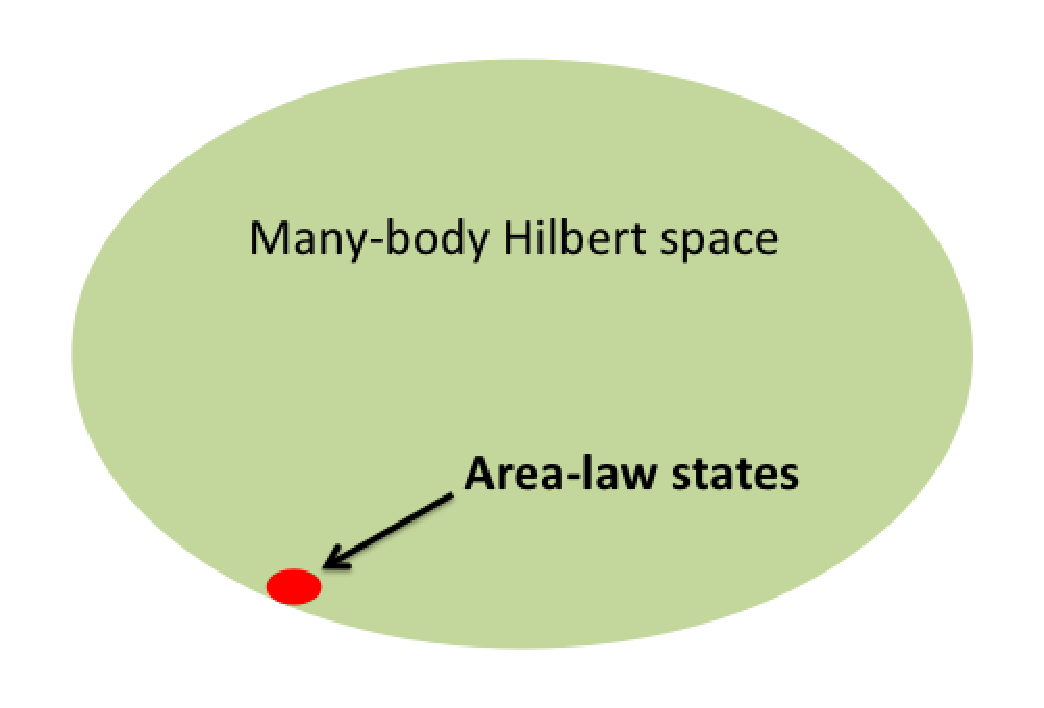
\includegraphics[width=0.9\textwidth]{orus-images/fig4.pdf}
            \end{figure}}
        \end{column}
\end{columns}   


\end{frame}

\begin{frame}{Why tensor networks?}
    \bi
    \item <1-> Tensor networks algorithms generalize renormalization group methods
    \bi
    \item <2-> Numerical RG (Wilson)
    \begin{figure}[htbp]
               \scalebox{0.6}{ %!TEX root = ../thesis.tex

\beginpgfgraphicnamed{mps1}
\begin{tikzpicture}[node distance=0.5cm]

\foreach \i in {1,2,3,4,5,6}
{
	\node[spin] (s\i) at (\i,0) {};
	\node[below of=s\i] {$H_\i$};
}

\foreach \i / \j in {1/2,2/3,3/4,4/5,5/6}
{
	\node[gamma] (g\i) at (\i+0.5,0.5*\i) {};
	\node[above left of=g\i] {$A_\i$};
%	\draw let \n1={\i+1} in (g\i) -- (s\n1);
	\draw (g\i) -- (s\j);
}

\foreach \i / \j in {2/1,3/2,4/3,5/4}
{
%	\draw let \n1={\i-1} in (g\i) -- (g\n1);
	\draw (g\i) -- (g\j);
}

\draw (s1) -- (g1);
\draw (g5) -- ($ (g5) + (0.5,0.5) $);

\end{tikzpicture}}
            \end{figure}
    \ei
    \item <3-> Interesting physical systems can be described by simple tensor networks
    \bi
    \item <4-> Including non-chiral topological or SPT order
    \ei
    \ei
\end{frame}

%%%%%%%%%%%%%%%%%%%%%%%%%%%%%%%%%%%%%%%%%
%%%%%%%%%% Outline code %%%%%%%%%%%%%%%%%
%%%%%%%%%%%%%%%%%%%%%%%%%%%%%%%%%%%%%%%%%
\section*{}
\begin{frame}
  \frametitle{Outline}
  \tableofcontents[section=1,hidesubsections]
\end{frame}

\AtBeginSection[]
{
  \frame<handout:0>
  {
    \frametitle{Outline}
    \tableofcontents[currentsection,hideallsubsections]
  }
}

\AtBeginSubsection[]
{
  \frame<handout:0>
  {
    \frametitle{Outline}
    \tableofcontents[sectionstyle=show/hide,subsectionstyle=show/shaded/hide]
  }
}
%%%%%%%%%%%%%%%%%%%%%%%%%%%%%%%%%%%%%%%%%
%%%%%%%%%% Content starts here %%%%%%%%%%
%%%%%%%%%%%%%%%%%%%%%%%%%%%%%%%%%%%%%%%%%



\section{What is a tensor network?}

\begin{frame}{Frame Title}
\vskip-1.5cm

\end{frame}

\section{AKLT: the canonical MPS}

\begin{frame}{Frame Title}
\vskip-1.5cm

\end{frame}

\section{Constructing the toric code state}

\begin{frame}{Frame Title}
\vskip-1.5cm

\end{frame}

\section*{}

\frame{
  \vspace{2cm}
  {\huge Questions?}

  \vspace{3cm}
  \begin{flushright}
    Brayden Ware

    \structure{\footnotesize{brayden@physics.ucsb.edu}}
  \end{flushright}
}

\frame{
  \vfill
  \centering
  \highlighton{
  \usebeamerfont*{frametitle}Bonus slides

  %\usebeamerfont*{framesubtitle}Bonus slides
  }
  \vfill
}

\begin{frame}
  \frametitle{Resources}
  \vskip-1.7cm
  %\framesubtitle{If you want to improve this style}
  \bibliography{references}
  %\beamertemplatearticlebibitems
\end{frame}



\end{document}
